\begin{figure}[htbp]
\centering
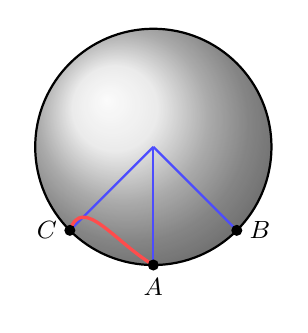
\begin{tikzpicture}
\shade[ball color=gray!25,opacity=0.85] (0,0) circle (1.5);
\draw[thick] (0,0) circle (1.5);
\draw[thick,blue!70] (0,0) -- (0,-1.5);
\draw[thick,blue!70] (0,0) -- (1.06,-1.06);
\draw[thick,blue!70] (0,0) -- (-1.06,-1.06);
\draw[very thick,red!70] (0,-1.5) .. controls (-0.5,-1.2) and (-0.9,-0.6) .. (-1.06,-1.06);
\fill (0,-1.5) circle (2pt);
\fill (1.06,-1.06) circle (2pt);
\fill (-1.06,-1.06) circle (2pt);
\node[below] at (0,-1.55) {\small $A$};
\node[right] at (1.1,-1.05) {\small $B$};
\node[left] at (-1.1,-1.05) {\small $C$};
\end{tikzpicture}
\caption{球面上的平行移动：矢量从 $A$ 沿大圆挪到 $B$、再到 $C$、最后回到 $A$。绕一圈回来，方向变了——角度差等于这三点大圆三角形的面积（以 $a^2$ 为单位）。这个「挪一圈回不来」正是曲率。}
\end{figure}
